\documentclass[11pt, paper=a4]{article}
\usepackage[left=4.5cm, right=4.5cm, top=2cm, bottom=3cm %showframe
]{geometry}

\usepackage{amsmath}
\usepackage{amsthm}       
\usepackage{amssymb}

\usepackage{graphicx}

\newcommand{\E}{\operatorname{\mathbf{E}}}
\newcommand{\Var}{\operatorname{\mathbf{Var}}}

\addtolength{\parskip}{\baselineskip}
\parindent 0pt

\makeatletter
\renewcommand{\fnum@figure}{\figurename~S\thefigure}
\makeatother

\begin{document}

\begin{center}
  \Large
  Supporting Information for \textit{Non-random network connectivity comes in pairs}
  \smallskip
  \normalsize
  
  Felix Z.~Hoffmann, Jochen Triesch
\end{center}

\section*{SI1}

Solving
\begin{align}
\mu = px + (1-p)y
\end{align}
for $p$ gives
\begin{align}
  p = \frac{\mu-y}{x-y},
\end{align}
%
which, plugged into
\begin{align}
  \varrho = \frac{p x^2 + (1-p) y^2}{\mu^2},
\end{align}
yields
\begin{align}
  \varrho & = \frac{\left(\frac{\mu-y}{x-y}\right)x^2  + \left(1-\frac{\mu-y}{x-y}\right) y^2}{\mu^2} \\
  & = \frac{\left(\frac{\mu-y}{x-y}\right)(x^2-y^2) + y^2}{\mu^2}\\
  & = \frac{(\mu -y) (x+y) + y^2}{\mu^2} \\
  & = \frac{x+y}{\mu} - \frac{xy}{\mu^2}.
\end{align}

\section*{SI2}
Solve
\begin{align}
  p = \frac{\mu-y}{x-y}
\end{align}
for $y$ and since $x \geq \mu$,
\begin{align}
y = \frac{\mu - px}{1-p} \leq \frac{\mu - p\mu}{1-p} = \mu.
\end{align}

%% \section*{Figure S1}

\begin{figure}[h!]
\centering
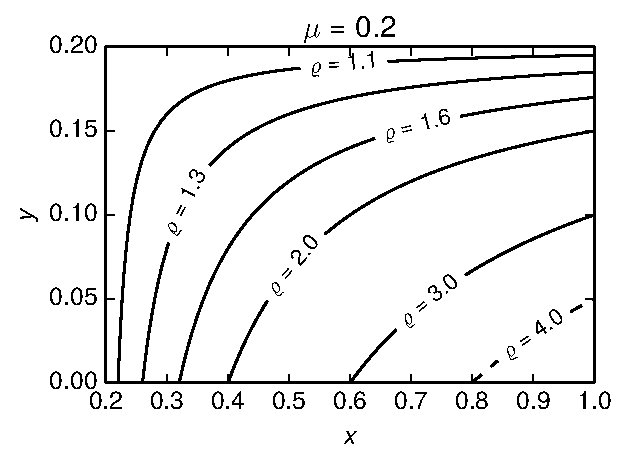
\includegraphics[width=0.7\textwidth]{%
  img/two_point_contour_mu02.pdf}
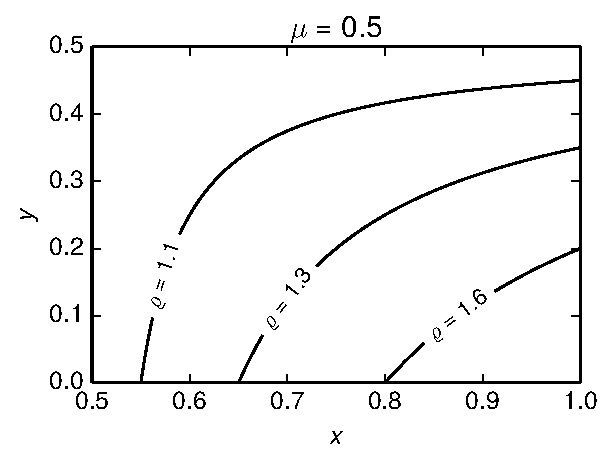
\includegraphics[width=0.67\textwidth]{%
  img/two_point_contour_mu05.pdf}
\caption{Relative overrepresentation $\varrho$ of bidirectional
  connections in networks with a fraction of pairs connected with a
  high probability $x$ and the rest of the pairs connected with a low
  probability $y$. \textbf{Top} Overall connection probability in the network $\mu = 0.2$ \textbf{Bottom} $\mu =0.5$ }
\label{fig:tp}
\end{figure}




\end{document}

